\section{An�lisis}\label{sec:analysis}

\subsection{}

Las figuras~\ref{fig:S1L1},~\ref{fig:S1L2} y~\ref{fig:S1L3} representan la relaci�n $\Delta V$ frente a $I$ para el primer cable
para las 3 longitudes.

De igual modo, las figuras~\ref{fig:S2L1},~\ref{fig:S2L2} y~\ref{fig:S2L3} corresponden al segundo cable y
las~\ref{fig:S3L1},~\ref{fig:S3L2} y~\ref{fig:S3L3}
al tercero.

\begin{figure}[h!]
    \begin{center}
        \includegraphics[width=0.8\columnwidth]{files/images/S1L1}
    \end{center}
    \caption{$\Delta V$ frente a $I$, cable $S = 1.5\,$mm$^2$ y $L = 1\,$m.}
    \label{fig:S1L1}
\end{figure}

\begin{figure}[h!]
    \begin{center}
        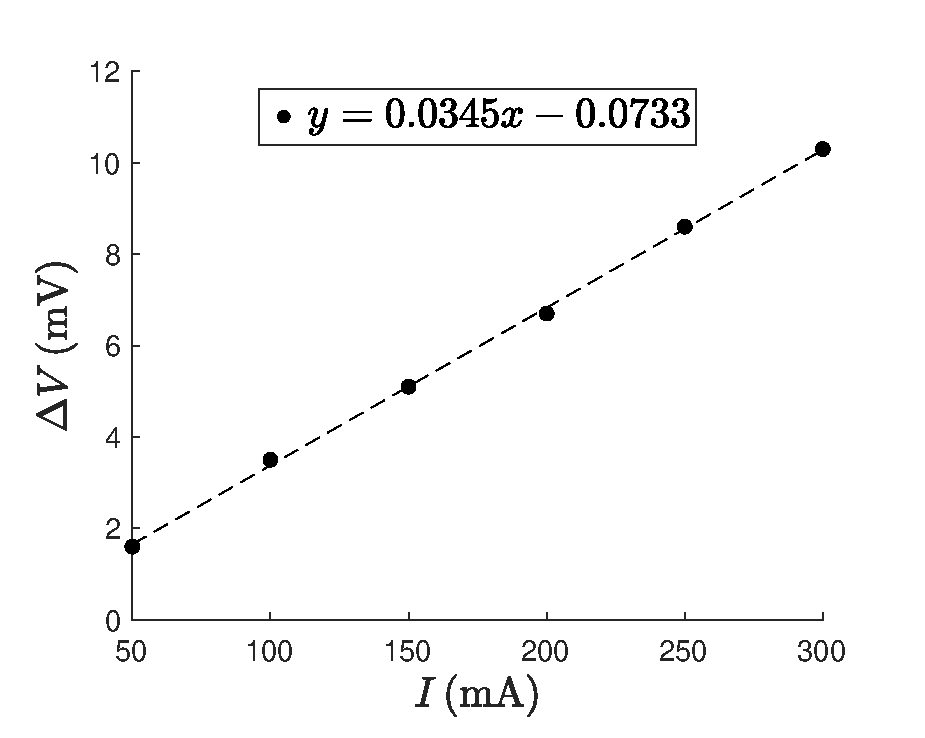
\includegraphics[width=0.8\columnwidth]{files/images/S1L2}
    \end{center}
    \caption{$\Delta V$ frente a $I$, cable $S = 1.5\,$mm$^2$ y $L = 1.5\,$m.}
    \label{fig:S1L2}
\end{figure}

\begin{figure}[h!]
    \begin{center}
        \includegraphics[width=0.8\columnwidth]{files/images/S1L3}
    \end{center}
    \caption{$\Delta V$ frente a $I$, cable $S = 1.5\,$mm$^2$ y $L = 2\,$m.}
    \label{fig:S1L3}
\end{figure}

\begin{figure}[h!]
    \begin{center}
        \includegraphics[width=0.8\columnwidth]{files/images/S2L1}
    \end{center}
    \caption{$\Delta V$ frente a $I$, cable $S = 0.5\,$mm$^2$ y $L = 1\,$m.}
    \label{fig:S2L1}
\end{figure}

\begin{figure}[h!]
    \begin{center}
        \includegraphics[width=0.8\columnwidth]{files/images/S2L2}
    \end{center}
    \caption{$\Delta V$ frente a $I$, cable $S = 0.5\,$mm$^2$ y $L = 1.5\,$m.}
    \label{fig:S2L2}
\end{figure}

\begin{figure}[h!]
    \begin{center}
        \includegraphics[width=0.8\columnwidth]{files/images/S2L3}
    \end{center}
    \caption{$\Delta V$ frente a $I$, cable $S = 0.5\,$mm$^2$ y $L = 2\,$m.}
    \label{fig:S2L3}
\end{figure}

\begin{figure}[h!]
    \begin{center}
        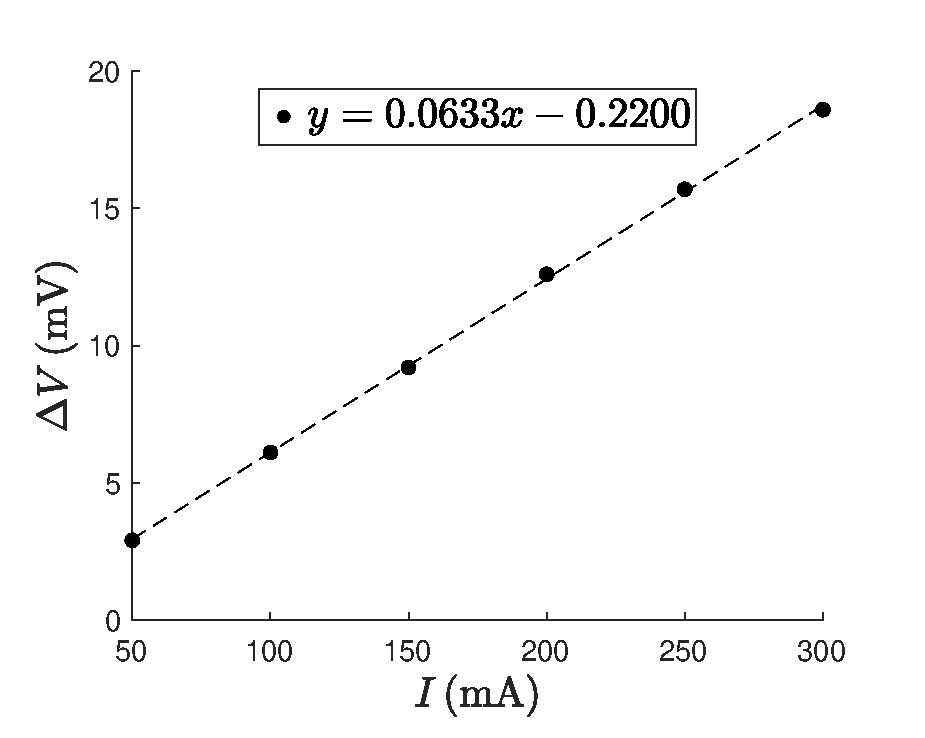
\includegraphics[width=0.8\columnwidth]{files/images/S3L1}
    \end{center}
    \caption{$\Delta V$ frente a $I$, cable $S = 0.325\,$mm$^2$ y $L = 1\,$m.}
    \label{fig:S3L1}
\end{figure}

\begin{figure}[h!]
    \begin{center}
        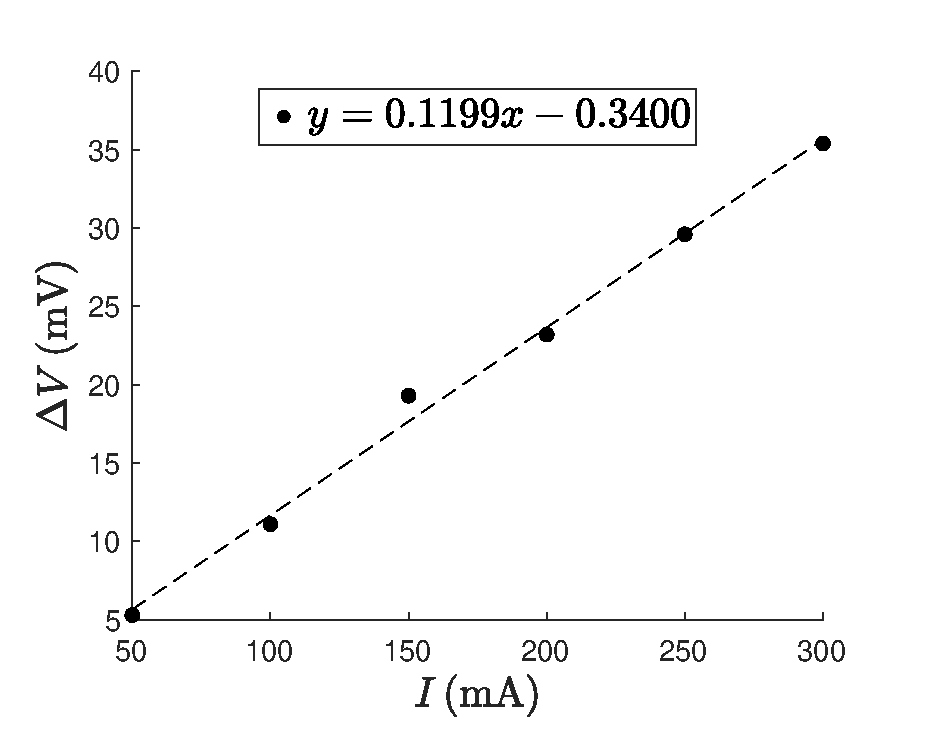
\includegraphics[width=0.8\columnwidth]{files/images/S3L2}
    \end{center}
    \caption{$\Delta V$ frente a $I$, cable $S = 0.32\,$mm$^2$ y $L = 1.5\,$m.}
    \label{fig:S3L2}
\end{figure}

\begin{figure}[h!]
    \begin{center}
        \includegraphics[width=0.8\columnwidth]{files/images/S3L3}
    \end{center}
    \caption{$\Delta V$ frente a $I$, cable $S = 0.32\,$mm$^2$ y $L = 2\,$m.}
    \label{fig:S3L3}
\end{figure}

\FloatBarrier

La ordenada en el origen que se obtiene en el ajuste de los datos es el valor que corresponder�a a
la diferencia de potencial $\Delta V$ para una intensidad de corriente $I$ nula.

Idealmente, el valor de la ordenada en el origen deber�a ser 0.
El que no lo sea indica que en nuestras mediciones experimentales hemos
introducido un error.

Adem�s, la pendiente de las rectas es distinta en cada caso
porque la resistencia de cada cable var�a con la longitud $L$ y tambi�n con la secci�n $S$, seg�n la expresi�n~\ref{eq:ressitividad}.

\subsection{}

\FloatBarrier

